\begin{figure}[H]
    \centering
    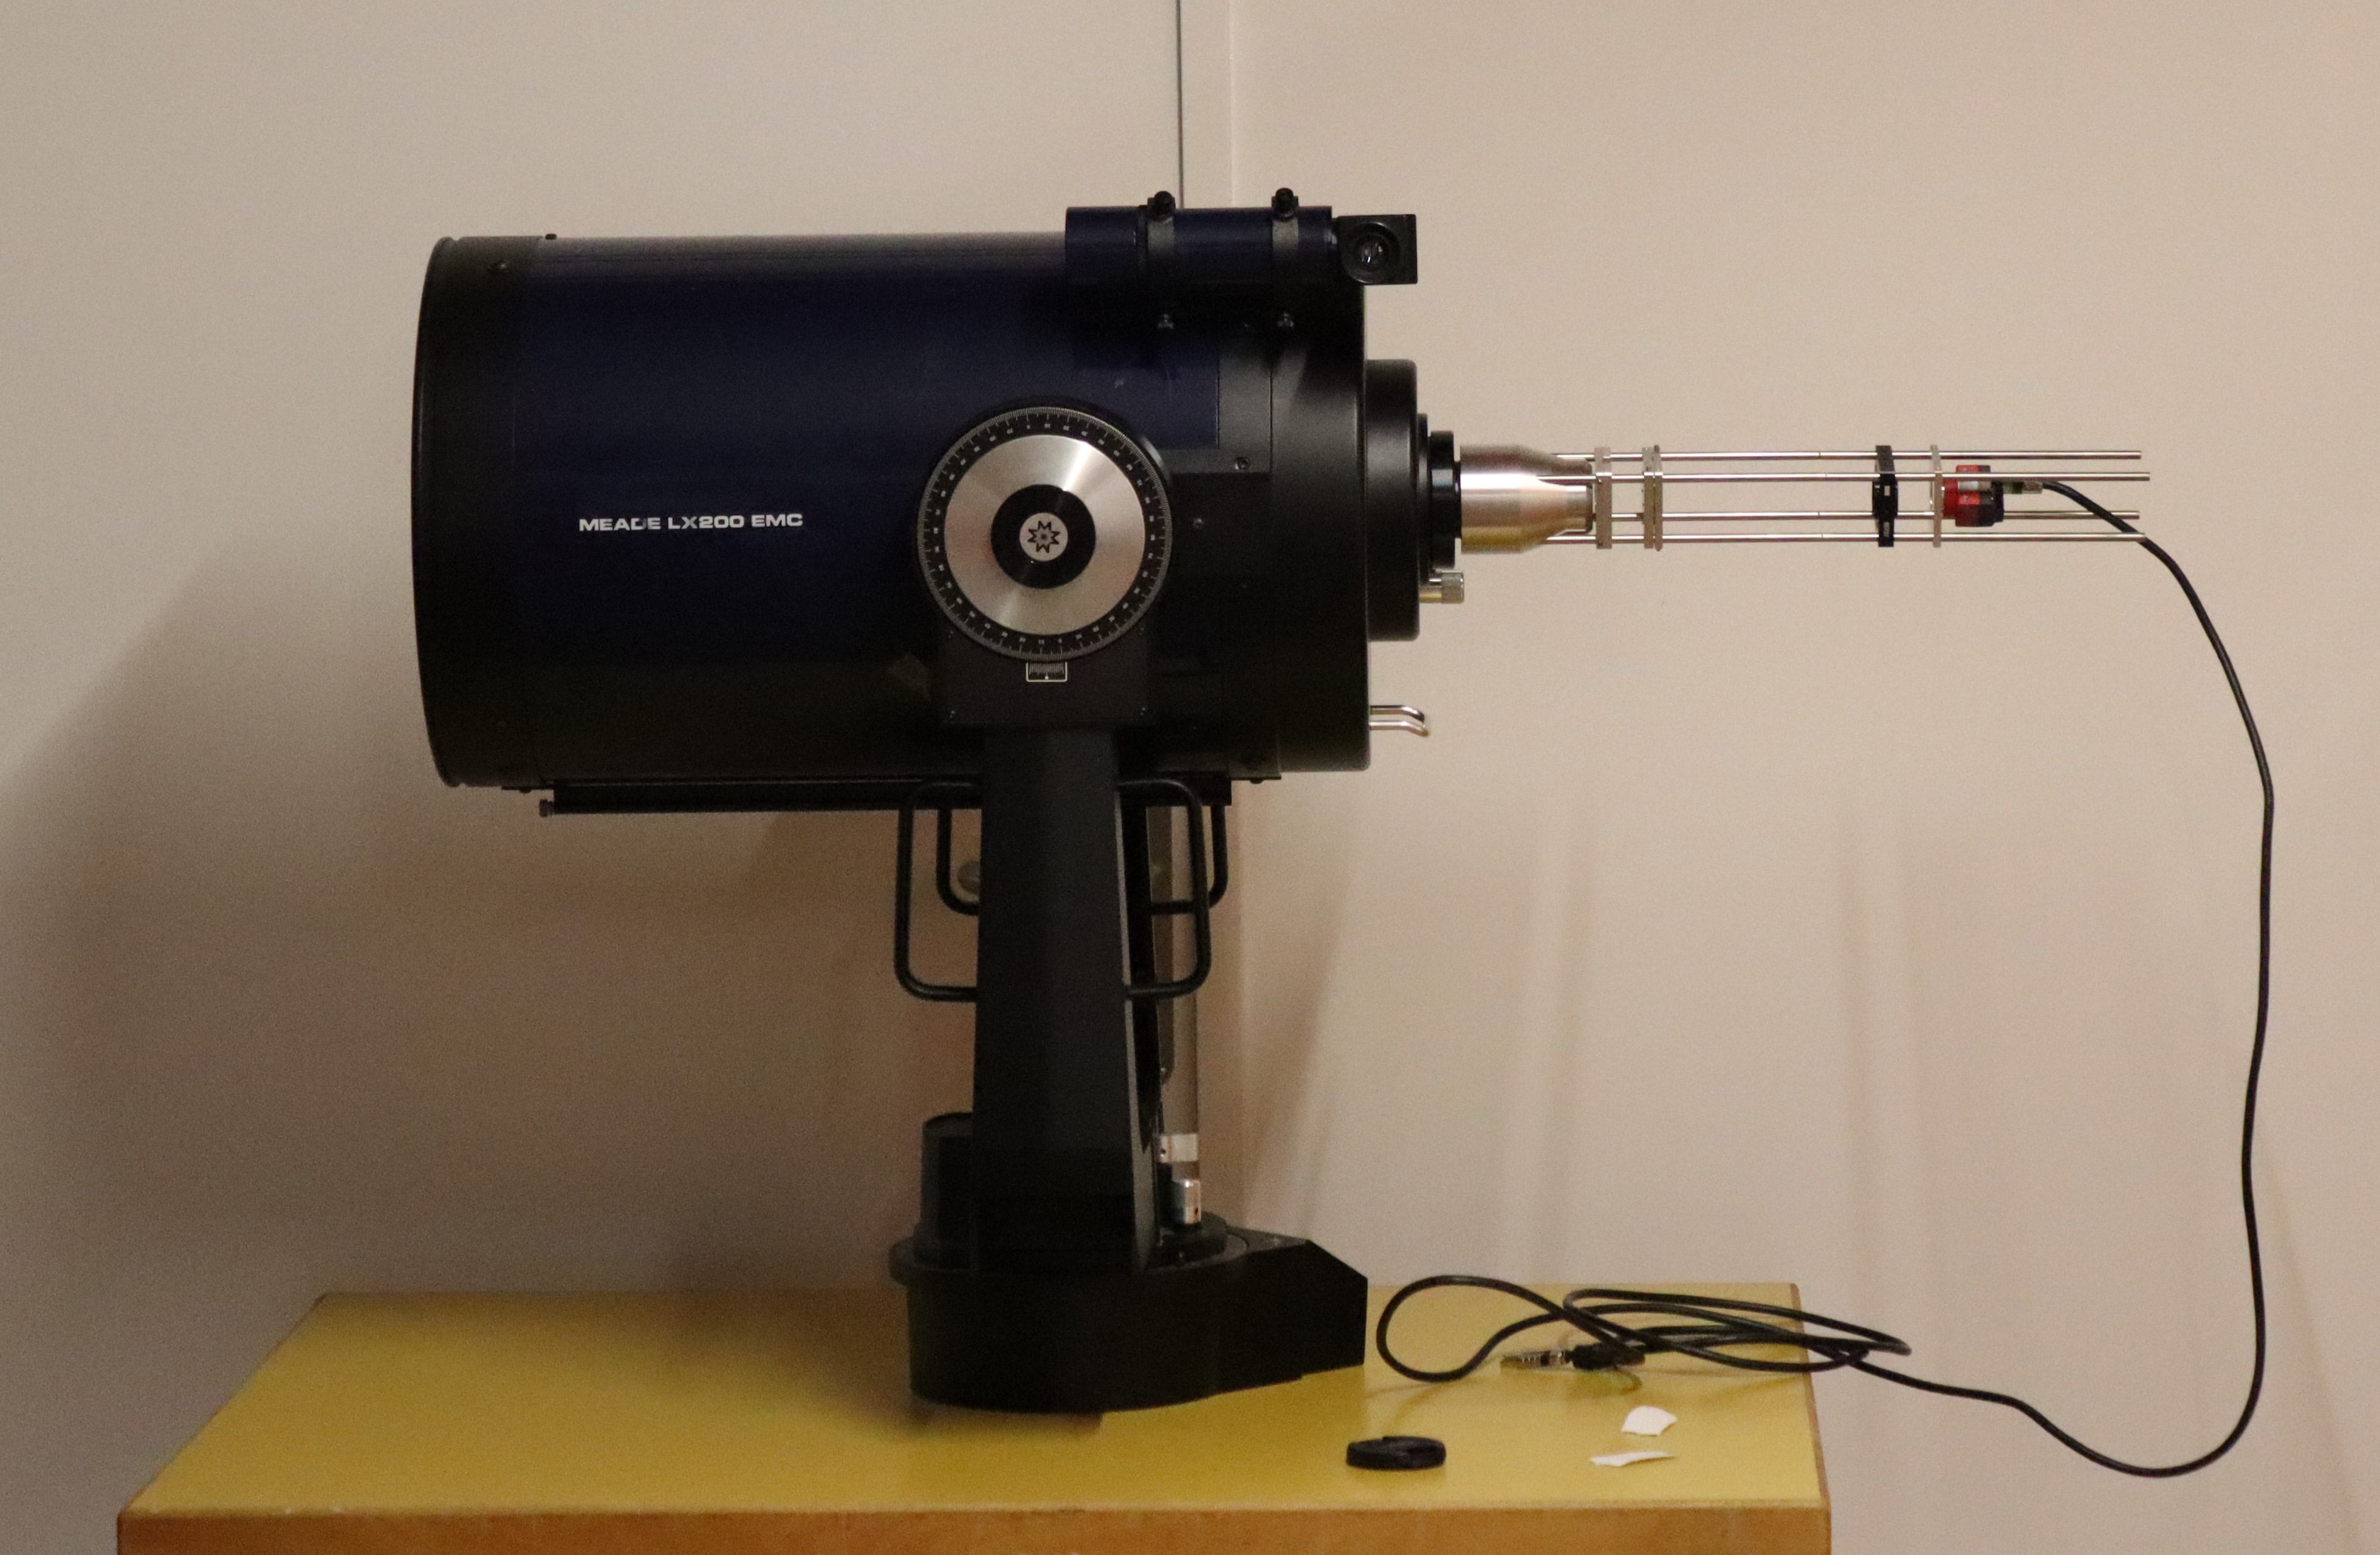
\includegraphics[scale=0.1]{assets/figures/System/IMG_5308.JPG}
    \caption{Mounted system}
    \label{fig:GLOB_Syst}
\end{figure}
\newpage
\section{System reports}
The telescope and mounted system can be seen in figure \ref{fig:GLOB_Syst}. 
The mechanical parts are well matched, and mounting the prisms and mask is easy. \newline
To attach the bars to the ocular holder, simply insert them into the holes provided. Screws (UNC 4-40 x 30) 
are required to secure them. 
\begin{figure}[H]
    \centering
    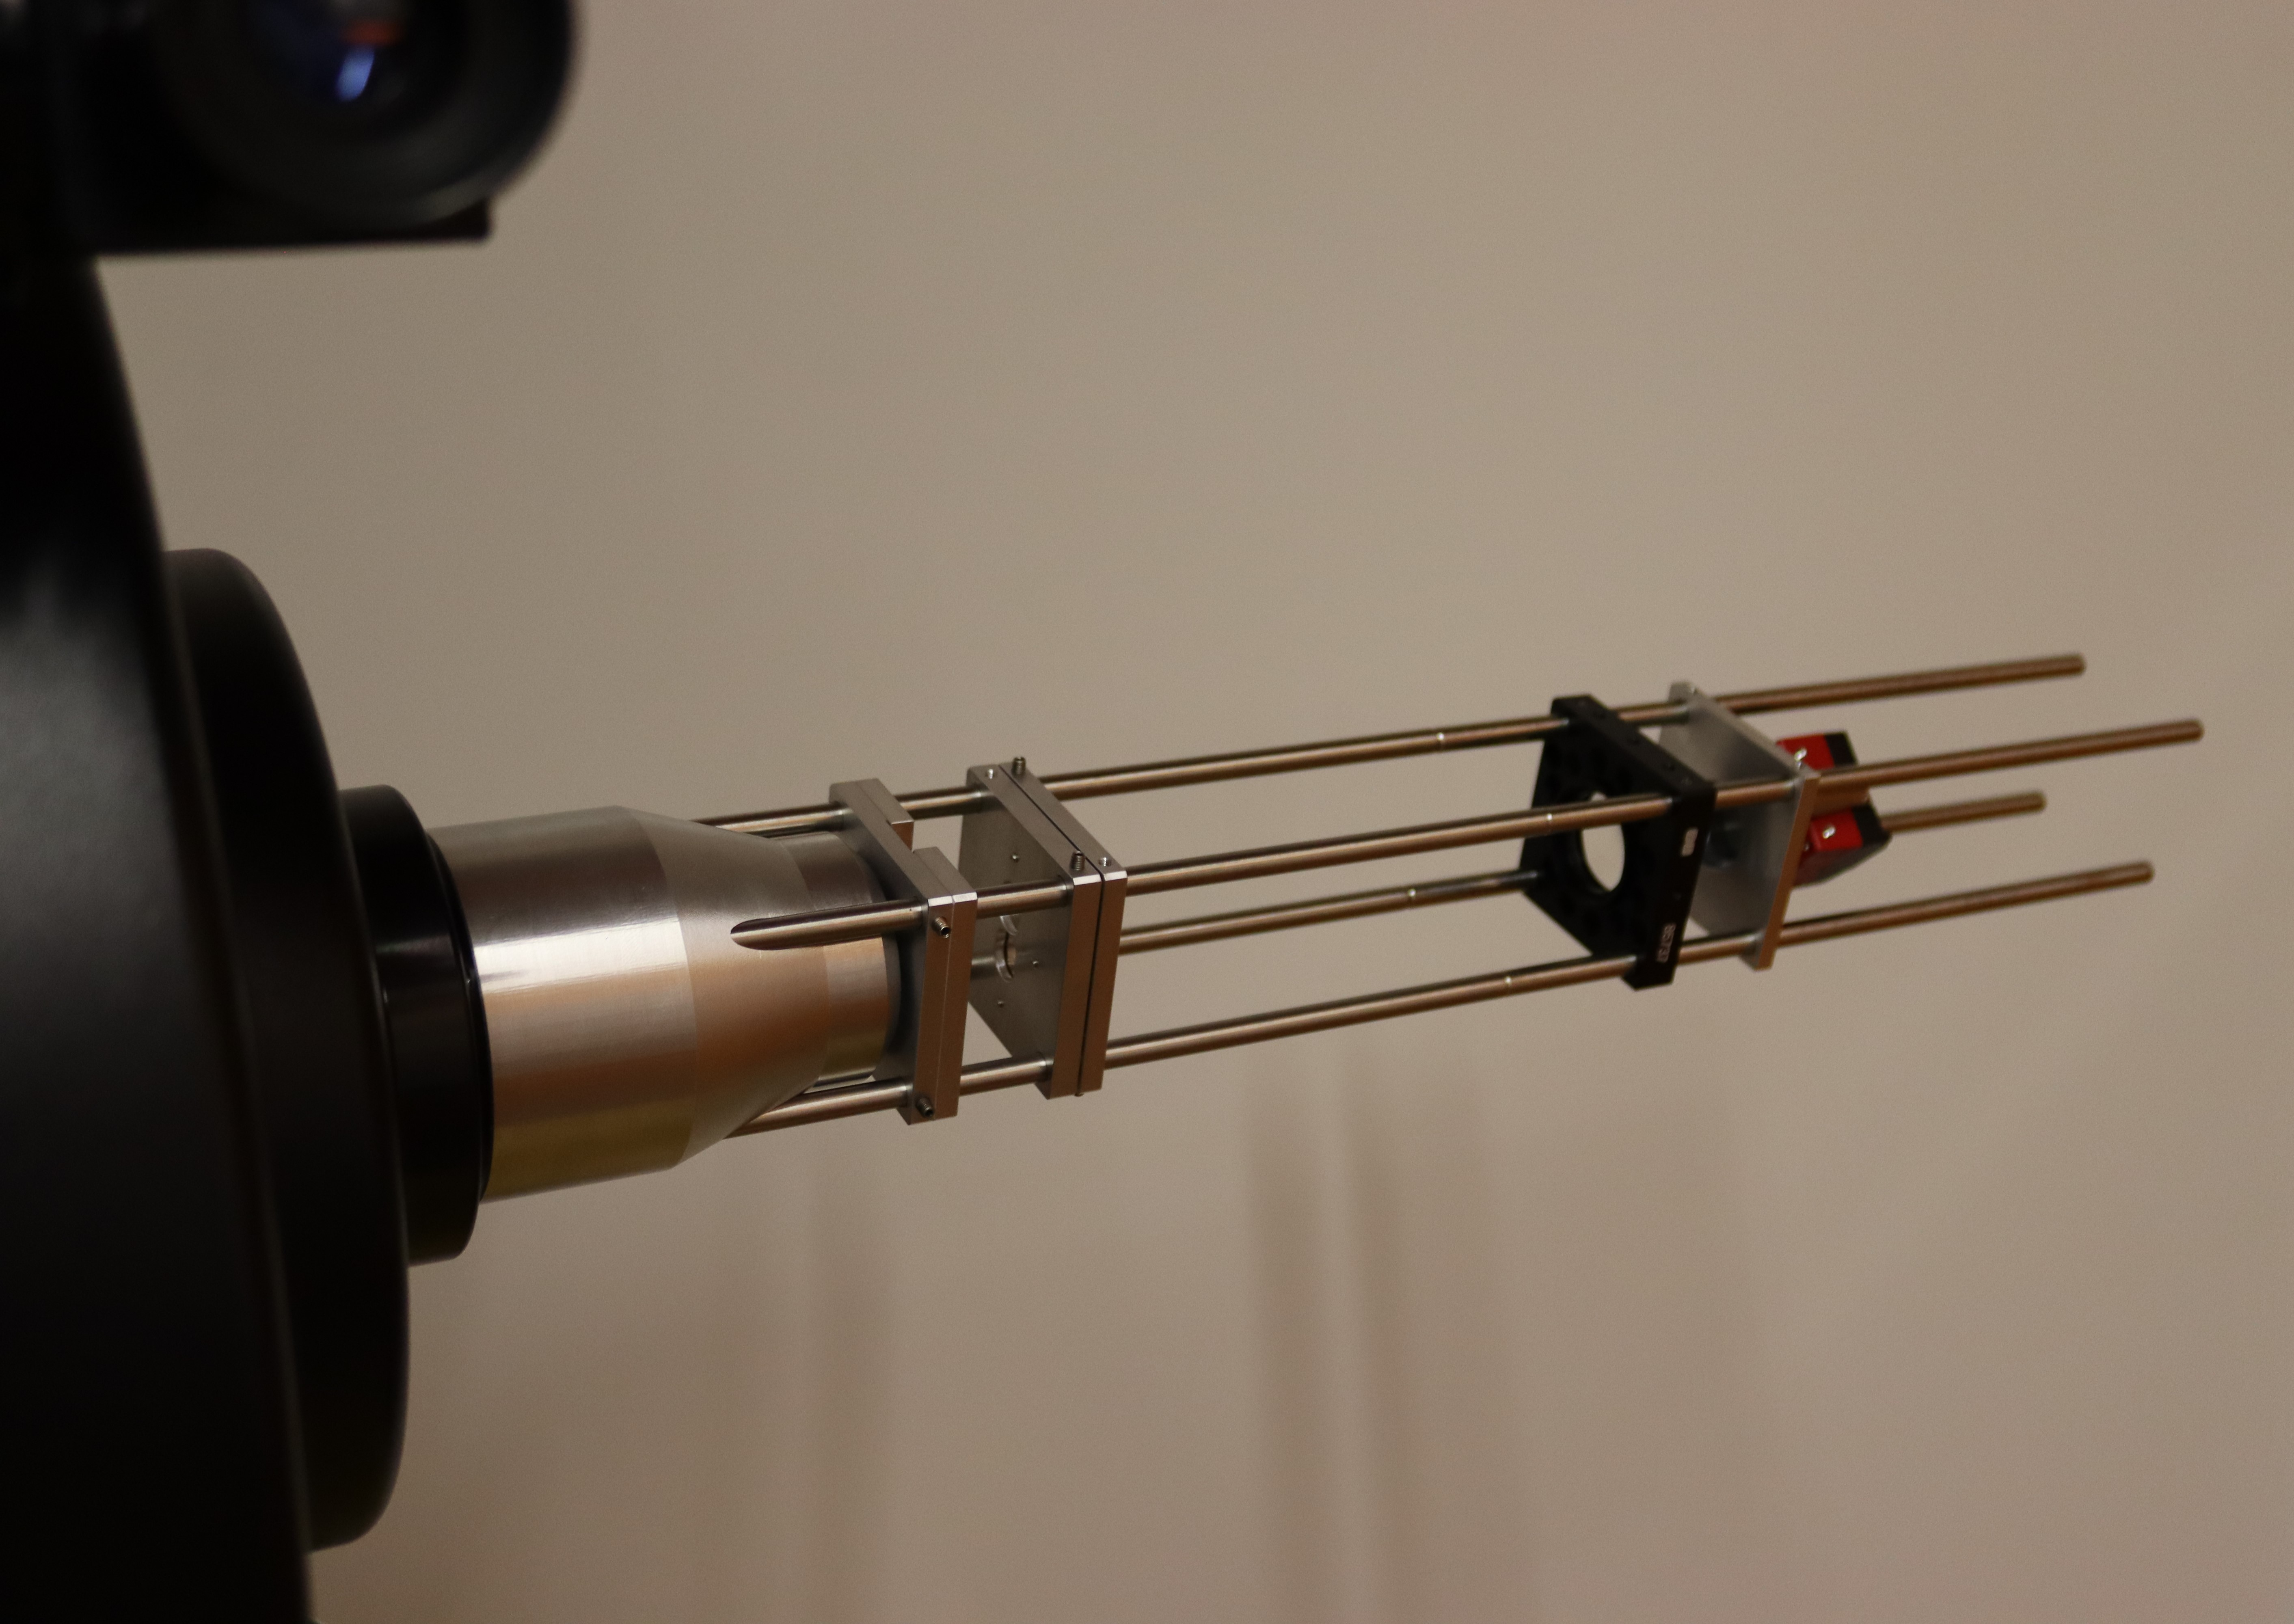
\includegraphics[scale=0.05]{assets/figures/System/IMG_5312.JPG}
    \caption{System rear view}
    \label{fig:GLOB_Barres}
\end{figure}
As shown in Figure \ref{fig:GLOB_Barres}, the assembly is based on 2 rods fastened together by grub screws. 
This choice was made for stock reasons. The only rods allowing this attachment were too short, 
so we had to put 2 of them one behind the other. 
This system works well for the experimental part, but it would be better to use a single bar over the whole system to 
avoid excessive bending and facilitate sliding of the elements.
\begin{figure}[H]
    \centering
    \includegraphics[scale=0.05]{assets/figures/System/IMG_5317.JPG}
    \caption{System front view}
    \label{fig:GLOB_JSP}
\end{figure}
\section{Instruction manual}
All the steps required to prepare the measurement are listed below. Steps 7 to 9 are not feasible at present, 
as the software has not yet been implemented in the user interface.
for the time being, as the software has not yet been implemented in the user interface. However, they can be replaced by capturing images with Vimba software. However, we have chosen to note them for future improvements.
\begin{enumerate}
    \item Install the ocular holder fitted with this on the telescope.
    \item Point the telescope at the star and position your eye against the occular.
    \item Adjust the telescope's focal length to see a sharp image.
    \item Installing the assembly (without mask).
    \item Connect the camera to the computer and, if necessary, check the image using Vimba software. 
    If the image is not sharp, adjust the lens so that the sensor is at its focal length.
    \item Insert mask into mask holder.
    \item Start "DIMM V1" software.
    \item Define the document where the results file will be stored and, if necessary, test the camera connection.
    \item Start the measurement and wait for the popup window to display the result.
\end{enumerate}
If the results are inconclusive or faulty, you can modify the camera parameters directly from the interface.
Image and data feedback is also available in this software.